\documentclass[10pt,a4paper,twoside,twocolumn]{scrartcl}
\usepackage[utf8]{inputenc}
\usepackage[T1]{fontenc}
\usepackage[brazil]{babel}
% Libertine e a fonte do boilerplate arabica
\usepackage{libertine}
\usepackage[libertine]{newtxmath}
\usepackage{microtype}
\usepackage{amsmath,amssymb}
\usepackage{booktabs,longtable,array,colortbl}
\usepackage{graphicx}
\usepackage{xcolor}
\usepackage{fancyvrb}
\usepackage{scrlayer-scrpage}
\usepackage[a4paper,margin=1.8cm,columnsep=0.75cm]{geometry}
\usepackage{setspace}
\setstretch{0.99}
% hyperref fica de fora: a versao instalada exige um kernel LaTeX mais novo que
% o do MiKTeX 23.10 desta maquina ("key property '.initial:e' is unknown")
\providecommand{\tightlist}{%
  \setlength{\itemsep}{0pt}\setlength{\parskip}{0pt}}
\providecommand{\pandocbounded}[1]{#1}
% substitutos do hyperref: o link nao fica clicavel, mas o texto aparece e a URL
% vai para a nota de rodape, entao nada se perde na versao impressa.
% O pacote url quebra endereco longo em varias linhas; sem ele a URL estoura a
% largura da coluna e invade a coluna vizinha.
% xurl quebra a URL em qualquer ponto; o pacote url so' quebra em pontuacao, e
% dominios longos ainda estouravam a coluna
\usepackage{xurl}
\urlstyle{tt}
% nota de rodape em coluna estreita: sem \sloppy o TeX prefere estourar a
% margem a quebrar a URL num ponto que ele considera ruim
\renewcommand{\href}[2]{#2\footnote{\raggedright\tiny\sloppy
  \hbadness=10000 \url{#1}}}
\providecommand{\phantomsection}{}
\providecommand{\hypertarget}[2]{#2}
\providecommand{\texorpdfstring}[2]{#1}
\providecommand{\citeproctext}{}

% macros de destaque de sintaxe (CommentTok, KeywordTok, ...) que o pandoc gera
% para os blocos de codigo; sem isto o Python do texto sai com comandos indefinidos
\usepackage{color}
\usepackage{fancyvrb}
\newcommand{\VerbBar}{|}
\newcommand{\VERB}{\Verb[commandchars=\\\{\}]}
\DefineVerbatimEnvironment{Highlighting}{Verbatim}{commandchars=\\\{\}}
% Add ',fontsize=\small' for more characters per line
\newenvironment{Shaded}{}{}
\newcommand{\AlertTok}[1]{\textcolor[rgb]{1.00,0.00,0.00}{\textbf{#1}}}
\newcommand{\AnnotationTok}[1]{\textcolor[rgb]{0.38,0.63,0.69}{\textbf{\textit{#1}}}}
\newcommand{\AttributeTok}[1]{\textcolor[rgb]{0.49,0.56,0.16}{#1}}
\newcommand{\BaseNTok}[1]{\textcolor[rgb]{0.25,0.63,0.44}{#1}}
\newcommand{\BuiltInTok}[1]{\textcolor[rgb]{0.00,0.50,0.00}{#1}}
\newcommand{\CharTok}[1]{\textcolor[rgb]{0.25,0.44,0.63}{#1}}
\newcommand{\CommentTok}[1]{\textcolor[rgb]{0.38,0.63,0.69}{\textit{#1}}}
\newcommand{\CommentVarTok}[1]{\textcolor[rgb]{0.38,0.63,0.69}{\textbf{\textit{#1}}}}
\newcommand{\ConstantTok}[1]{\textcolor[rgb]{0.53,0.00,0.00}{#1}}
\newcommand{\ControlFlowTok}[1]{\textcolor[rgb]{0.00,0.44,0.13}{\textbf{#1}}}
\newcommand{\DataTypeTok}[1]{\textcolor[rgb]{0.56,0.13,0.00}{#1}}
\newcommand{\DecValTok}[1]{\textcolor[rgb]{0.25,0.63,0.44}{#1}}
\newcommand{\DocumentationTok}[1]{\textcolor[rgb]{0.73,0.13,0.13}{\textit{#1}}}
\newcommand{\ErrorTok}[1]{\textcolor[rgb]{1.00,0.00,0.00}{\textbf{#1}}}
\newcommand{\ExtensionTok}[1]{#1}
\newcommand{\FloatTok}[1]{\textcolor[rgb]{0.25,0.63,0.44}{#1}}
\newcommand{\FunctionTok}[1]{\textcolor[rgb]{0.02,0.16,0.49}{#1}}
\newcommand{\ImportTok}[1]{\textcolor[rgb]{0.00,0.50,0.00}{\textbf{#1}}}
\newcommand{\InformationTok}[1]{\textcolor[rgb]{0.38,0.63,0.69}{\textbf{\textit{#1}}}}
\newcommand{\KeywordTok}[1]{\textcolor[rgb]{0.00,0.44,0.13}{\textbf{#1}}}
\newcommand{\NormalTok}[1]{#1}
\newcommand{\OperatorTok}[1]{\textcolor[rgb]{0.40,0.40,0.40}{#1}}
\newcommand{\OtherTok}[1]{\textcolor[rgb]{0.00,0.44,0.13}{#1}}
\newcommand{\PreprocessorTok}[1]{\textcolor[rgb]{0.74,0.48,0.00}{#1}}
\newcommand{\RegionMarkerTok}[1]{#1}
\newcommand{\SpecialCharTok}[1]{\textcolor[rgb]{0.25,0.44,0.63}{#1}}
\newcommand{\SpecialStringTok}[1]{\textcolor[rgb]{0.73,0.40,0.53}{#1}}
\newcommand{\StringTok}[1]{\textcolor[rgb]{0.25,0.44,0.63}{#1}}
\newcommand{\VariableTok}[1]{\textcolor[rgb]{0.10,0.09,0.49}{#1}}
\newcommand{\VerbatimStringTok}[1]{\textcolor[rgb]{0.25,0.44,0.63}{#1}}
\newcommand{\WarningTok}[1]{\textcolor[rgb]{0.38,0.63,0.69}{\textbf{\textit{#1}}}}

\definecolor{tinta}{HTML}{1a1a1a}
\definecolor{destaque}{HTML}{1f3a5f}   % azul-petroleo sobrio, no lugar do vermelho
\definecolor{linhatab}{HTML}{9aa4ad}
\definecolor{fundotab}{HTML}{eef1f4}
\color{tinta}

\setkomafont{disposition}{\normalfont\bfseries}
\addtokomafont{section}{\large}
\addtokomafont{subsection}{\normalsize}
% sem numeracao: e um relato, nao um artigo com referencia cruzada
\setcounter{secnumdepth}{0}
\setlength{\parindent}{0pt}
\setlength{\parskip}{0.35em}
\setlength{\emergencystretch}{3em}

% citacoes com cara de citacao: recuo, fio lateral e italico
\renewenvironment{quote}
  {\begin{list}{}{\leftmargin=0.9em\rightmargin=0pt\topsep=0.5em}\item[]%
   \color{destaque}\itshape\small
   \hspace*{-0.9em}\rule[-0.4em]{1.2pt}{1.1em}\hspace{0.5em}\ignorespaces}
  {\end{list}}

% codigo: menor e sempre dentro da coluna, com quebra automatica
\fvset{fontsize=\tiny,breaklines=true,breakanywhere=true,
       frame=leftline,framerule=0.8pt,rulecolor=\color{linhatab},
       xleftmargin=0.5em,framesep=0.5em}
% o pandoc gera \begin{verbatim} (do LaTeX puro), que NAO quebra linha e estoura
% a coluna. Redefinir para o Verbatim do fancyvrb faz o fvset acima valer.
\DefineVerbatimEnvironment{verbatim}{Verbatim}{}
\DefineVerbatimEnvironment{Highlighting}{Verbatim}{commandchars=\\\{\}}
\let\oldtexttt\texttt
\renewcommand{\texttt}[1]{{\small\oldtexttt{#1}}}

% tabelas fechadas, com regua mais forte e cabecalho destacado
\setlength{\aboverulesep}{0pt}\setlength{\belowrulesep}{0pt}
\setlength{\extrarowheight}{2pt}
\renewcommand{\arraystretch}{1.12}
\arrayrulecolor{linhatab}
\pagestyle{scrheadings}
\clearpairofpagestyles
\ohead{\small\itshape Pinball, Paciência e um Viking}
\ofoot*{\small\pagemark}

% imagens e tabelas nunca passam da largura da coluna
\makeatletter
\def\maxwidth{\ifdim\Gin@nat@width>\linewidth\linewidth\else\Gin@nat@width\fi}
\makeatother
\setkeys{Gin}{width=\maxwidth,keepaspectratio}

% referencias: o citeproc do pandoc gera esta lista
\newlength{\cslhangindent}\setlength{\cslhangindent}{1.5em}
\newlength{\csllabelwidth}\setlength{\csllabelwidth}{3em}
\newenvironment{CSLReferences}[2]{\small\setlength{\parindent}{0pt}%
  \everypar{\hangindent=\cslhangindent\hangafter=1}}{\par}
\newcommand{\CSLBlock}[1]{#1\hfill\break}
\newcommand{\CSLLeftMargin}[1]{\parbox[t]{\csllabelwidth}{#1}}
\newcommand{\CSLRightInline}[1]{\parbox[t]{\linewidth - \csllabelwidth}{#1}}
\newcommand{\CSLIndent}[1]{\hspace{\cslhangindent}#1}

\title{\Huge Pinball, Paciência e um Viking}
\subtitle{\normalsize Como treinar um agente de aprendizado por reforço
no 3D Pinball me fez descobrir que eu estava medindo a coisa errada}
\author{Adriano Pires Cunha}
\date{Agosto de 2026}

\begin{document}
\twocolumn[
  \begin{@twocolumnfalse}
  \maketitle
  \begin{abstract}
  \noindent Relato de quinze passos de experimento treinando um agente
de aprendizado por reforço no 3D Pinball Space Cadet do Windows XP,
sobre a decompilação em C++ do jogo instrumentada para expor o estado
interno da física. O agente alcança 2,6 milhões de pontos, 4,3 vezes uma
política aleatória, mas com 250 ms de latência de ação, na faixa usada
como referência humana, cai para 0,62 vezes o acaso: a vantagem é
reflexo, não estratégia. Mais de dez intervenções distintas falharam em
mover o teto, e a ordem por pontuação mostrou-se idêntica à ordem por
tempo de sobrevivência em todas.
  \end{abstract}
  \vspace{1.2em}
  \end{@twocolumnfalse}
]

\section{Tudo começou com um
viking}\label{tudo-comeuxe7ou-com-um-viking}

Eu queria mudar a cara de um personagem.

É sério, foi só isso. Instalei o 3D Pinball Space Cadet, aquele do
Windows XP, por pura saudade. Abri, joguei duas partidas, perdi as duas,
e reparei que o piloto da nave no canto da tela era um bonequinho
genérico de capacete.

E aí veio a associação boba que dá origem a projetos inteiros. Eu tinha
visto \emph{Freaks and Geeks} (Feig; Apatow, 1999), aquele episódio em
que o Sam tenta impressionar a Cindy, e a série tem um viking que ficou
na minha cabeça. Olhei o piloto do pinball e pensei que ele ficaria
melhor de elmo e barba.

Não existe motivo racional para isso. Eu estava com tempo livre e queria
ver um viking pilotando uma nave espacial num jogo de 1995.

\begin{figure}[tb]\centering
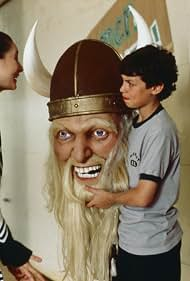
\includegraphics[width=4.6cm]{img/freaks_geeks.jpg}
\caption{A referência que começou tudo: o viking de \emph{Freaks and Geeks}.}
\end{figure}

O arquivo do jogo é um \texttt{PINBALL.DAT} de formato proprietário, sem
documentação oficial, cheio de bitmaps colados uns nos outros. Escrevi
um parser e descobri que os 318 bitmaps compartilham uma paleta global
de 256 cores: mexer numa entrada estraga a mesa inteira. Sobravam 19
índices livres, e trabalhei dentro deles.

Depois de umas cinco tentativas de desenhar o viking por código, o
resultado estava tão ruim que eu ri sozinho. Barba grande demais, elmo
flutuando acima da cabeça, resquícios do capacete antigo aparecendo por
trás. Parecia um acidente industrial. Desisti da abordagem, gerei a
imagem que eu queria num modelo de imagem, e escrevi um conversor:
alinhamento por busca de escala e deslocamento, requantização com
distância perceptual, preenchimento por vizinhança para não deixar
buraco no fundo com dither.

\begin{figure*}[tb]\centering
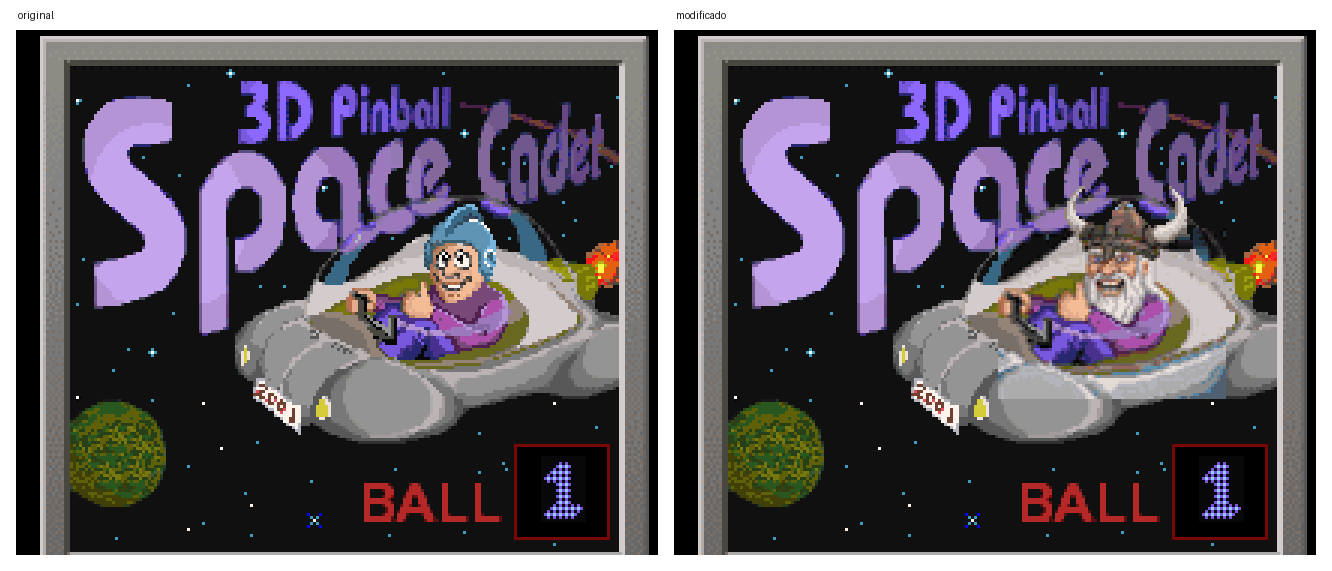
\includegraphics[width=13cm]{img/viking_no_jogo.png}
\caption{O jogo rodando com o arquivo original e com o modificado. São 70 por
57 pixels de sprite, trocados dentro da paleta global de 256 cores.}
\end{figure*}

Funcionou. O viking ficou lá, pilotando a nave. E foi aí que a coisa
saiu do controle.

Foi um vídeo que ligou uma coisa na outra.

Por essa época eu estava vendo um vídeo do Simon, \emph{Mastering the
Hex: A Case Study in Reinforcement Learning for Strategy Games} (Simon,
2026), sobre treinar uma inteligência artificial para jogar Antiyoy, um
jogo de estratégia hexagonal. O vídeo é ótimo e tem um detalhe que ficou
na minha cabeça: para treinar o agente, ele precisou \textbf{recriar o
jogo inteiro em Pygame}, porque o original era Java e não dava para
instrumentar.

Ele reconstruiu mecânica por mecânica, com o risco extra de a recriação
não bater com o jogo real.

Eu tinha acabado de passar um bom tempo dentro do formato binário do
Space Cadet. E pensei: \emph{``espera aí. O Space Cadet tem decompilação
em C++. O código-fonte reconstruído está no GitHub. Eu não preciso
recriar nada.''}

Foi essa a ideia. Pegar um jogo que praticamente todo brasileiro da
minha idade abriu pelo menos uma vez enquanto esperava alguma coisa
carregar, e transformar ele num laboratório de aprendizado por reforço
de verdade. Decidi embarcar nisso, e fui registrando o caminho enquanto
acontecia, que é o que você está lendo.

Aviso desde já: \textbf{o agente não bateu o recorde do jogo.} Ele
chegou a 2,6 milhões de pontos, e o recorde humano é 126 milhões. Está
48 vezes longe.

Mas a pergunta que este projeto acabou respondendo é bem mais
interessante do que ``dá para bater o recorde?'', e eu só cheguei nela
porque quase tudo que tentei deu errado primeiro.

\section{Antes de escrever código, uma boa
pesquisa}\label{antes-de-escrever-cuxf3digo-uma-boa-pesquisa}

Com o viking no lugar, a pergunta mudou: dá para fazer mais do que
trocar um sprite nesse jogo?

Minha primeira reação foi abrir o editor e começar. Segurei. Se a ideia
fosse boa, provavelmente alguém já tinha feito, e eu ia querer saber o
que essa pessoa aprendeu antes de repetir os erros dela.

Vale a pena listar o que encontrei, porque quase tudo aqui é útil para
quem quiser mexer com o mesmo jogo.

\textbf{\href{https://github.com/k4zmu2a/SpaceCadetPinball}{k4zmu2a/SpaceCadetPinball}}
é a peça central de tudo. É a decompilação em C++ do binário original do
Windows XP, feita por engenharia reversa, e ela \textbf{compila e roda}
({k4zmu2a}, 2021). Todo este projeto existe por causa desse repositório.
Sem ele eu estaria no mesmo barco do Simon, recriando pinball em Pygame.

\textbf{\href{https://github.com/AdrienTD/PinballTools}{AdrienTD/PinballTools}}
traz ferramentas de modding e, mais importante, documentação do formato
dos arquivos. Foi o que me ajudou no viking (Delahaye, 2020).

\textbf{\href{https://cryoganix.itch.io/3d-pinball-mod-tool}{3D Pinball
Mod Tool}} é uma interface gráfica de modding no itch.io, para quem não
quer escrever parser (Cryoganix, 2022).

Agora a parte que me interessava de verdade: alguém já tinha treinado IA
nesse jogo?

\textbf{\href{https://github.com/ElliotWood/3DPinballAI}{ElliotWood/3DPinballAI}}
usa Unity ML-Agents. Dez estrelas, arquivado em abril de 2020. Mas tem
um detalhe: é uma \textbf{recriação do jogo em Unity}, não o jogo
original. As físicas são do Unity, não do Space Cadet (Wood, 2020).

\textbf{\href{https://github.com/angelowilliams/space-cadet-nn}{angelowilliams/space-cadet-nn}}
usa algoritmo genético com captura de tela (OpenCV e MSS, a 30 quadros
por segundo). Nove estrelas (Williams, 2019). O README dele tem uma
frase que me pegou:

\begin{quote}
não roda em emulador nem é open source
\end{quote}

Era verdade quando ele escreveu, em 2019. Deixou de ser verdade com a
decompilação. E ninguém voltou para refazer o trabalho.

\textbf{\href{https://www.sumsar.net/blog/modeling-my-pinball-scores/}{Modeling
my pinball scores}}, do Rasmus Bååth, é modelagem bayesiana de pontuação
de pinball em R. Não é RL, mas é o precedente do lado estatístico, e me
deu ideias de como tratar a distribuição de score, que tem uma cauda
pesada horrorosa (Bååth, 2016).

Achei também os ports do jogo para Emscripten, Vita, Switch, Wii U,
libretro e PowerPC. Não usei nenhum, mas mostram o tamanho da comunidade
que ainda mexe nisso (Comunidade SpaceCadetPinball, 2024).

Já com o projeto adiantado, encontrei \textbf{Pinbot: Applying
Reinforcement Learning to Pinball Machines}, de Chaudhary, Mohta, Xiao,
Cuenca e Holand, do curso 16-831 da CMU, outono de 2024 (Chaudhary et
al., 2024). PPO sobre Visual Pinball X, mirando transferir o aprendizado
para uma máquina física de verdade.

Duas frases do paper deles descrevem, com outras palavras, coisas que eu
já tinha visto acontecer no meu:

\begin{quote}
o agente eventualmente aprendeu a simplesmente ficar parado sem lançar a
bola, com medo da penalidade futura quando a bola drenasse
\end{quote}

Isso é o meu primeiro treino, que colapsou em ``nunca apertar nada''.

\begin{quote}
uma recompensa simples baseada em tempo alcançaria um mínimo local onde
o agente simplesmente prende a bola no flipper
\end{quote}

Isso é o que eu vim a chamar de \textbf{berço}, e vou falar bastante
dele mais para frente.

Descobrir isso foi ótimo por dois motivos. Primeiro, tira meus achados
da categoria ``peculiaridade do Space Cadet'' e coloca como propriedade
do pinball enquanto problema de RL. Segundo, me deu a régua deles:

\vspace{0.2em}
\begin{center}\small
\resizebox{\ifdim\width>\linewidth\linewidth\else\width\fi}{!}{%
\begin{tabular}{|l|l|l|}
\hline
\rowcolor{fundotab}
& Score & Tempo \\
\hline
Humano & 38.952 & 69 s \\
\hline
Agente treinado & 33.952 & 57 s \\
\hline
Aleatório & 14.420 & 38 s \\
\hline
Sem agente & 8.358 & 36 s \\
\hline
\end{tabular}}
\end{center}
\vspace{0.1em}


O agente deles faz 2,35 vezes o aleatório e 87\% do humano. Esse segundo
número é o que eu não consigo calcular para o meu: volto a isso no
capítulo sobre latência.

Vale dimensionar o tamanho da coisa.

Sendo honesto sobre o tamanho da coisa: \textbf{instrumentar jogo de
código aberto para RL é técnica estabelecida desde o ViZDoom, em 2016}
(Kempka et al., 2016). Eu não inventei método nenhum.

O que eu faço aqui é preencher uma lacuna num nicho pequeno. Os dois
projetos de IA que existem para este jogo não usam o jogo real: um
recria em Unity, o outro fotografa a tela a 30 quadros por segundo.
Nenhum dos dois consegue ler o estado interno, e nenhum dos dois roda
mais rápido que tempo real.

O meu roda a \textbf{941 vezes a velocidade real} e lê a posição da bola
direto da física. Procurei bastante e não achei nada parecido: ninguém
tinha voltado ao jogo depois que a decompilação tornou isso possível.

É lacuna preenchida, não fronteira movida. Prefiro apresentar assim.

\section{O que significa instrumentar um
jogo}\label{o-que-significa-instrumentar-um-jogo}

Vale explicar isso direito, porque é a decisão técnica que define o
projeto inteiro.

Existem duas formas de fazer uma IA jogar um jogo.

\textbf{A forma de fora.} Você tira uma foto da tela, manda para uma
rede neural descobrir o que está acontecendo, e simula apertos de tecla.
É o que o space-cadet-nn faz. Funciona em qualquer jogo, inclusive nos
que você não tem o código. O preço é alto: você fica preso à velocidade
real, gasta processamento enorme convertendo pixels em significado, e o
agente precisa aprender a enxergar antes de aprender a jogar.

\textbf{A forma de dentro.} Você pega o código do jogo, acha a linha
onde ele calcula a posição da bola, e simplesmente \textbf{pergunta}. É
o que o ViZDoom fez com o Doom em 2016 (Kempka et al., 2016), e o que
virou padrão desde então.

A segunda é incomparavelmente melhor quando você tem o código. E eu
tinha.

Isso foi o que mais deu trabalho, porque não é óbvio. Depois de ler
bastante código, os pontos que importam são três:

A física roda a \textbf{120 Hz}, e eu agrupo três quadros por decisão: o
agente age a \textbf{40 Hz}, uma ação a cada 25 ms.

\texttt{pb::frame(float\ dt)} executa um passo de física. Chamar isso
num laço, sem desenhar nada na tela, é o que dá as 941 vezes a
velocidade real.

Esta chamada aplica o aperto do flipper, e é por aqui que o agente age:

\begin{verbatim}
MainTable->Message(
    MessageCode::LeftFlipperInputPressed,
    pb::time_now)
\end{verbatim}

\texttt{TPinballTable::CurScore} e a lista \texttt{BallList} dão o
placar e a bola. Estavam públicos, sem nenhum encapsulamento no caminho.

O código já separava física de renderização e já tinha modo de passo
único, o que sugere que quem fez a decompilação também precisou depurar
quadro a quadro.

Compilou de primeira. Escrevi um \texttt{rlenv.cpp} que roda o jogo numa
thread separada, com um handshake simples: o Python pede um passo, o C++
executa e devolve o estado. Um binding em pybind11 expõe isso para o
Python como um módulo normal.

Não é screenshot. É isto, direto da física, a cada 25 milissegundos:

\begin{verbatim}
bola_x, bola_y, bola_vx, bola_vy, bola_speed
score, bolas_restantes, bolas_em_jogo
rank, progresso, multiplicador
flip_esq_ang, flip_dir_ang
bola_rel_esq_x/y, bola_rel_dir_x/y
tilt, nudge_count
ev_bumper, ev_hyperspace, ev_medal,
ev_flip_acerto, ev_extra_ganha
\end{verbatim}

Os campos que começam com \texttt{ev\_} são contadores que eu
\textbf{adicionei ao C++}, incrementados dentro dos controladores do
jogo. Quando a bola bate num bumper, o contador sobe. Quando o flipper
em movimento toca a bola, outro contador sobe.

Esse último, o \texttt{ev\_flip\_acerto}, custou uma tarde e vai ser
importante mais para frente, então guarde o nome.

Uma armadilha que descobri no caminho: \texttt{TBall::ActiveFlag}
\textbf{não} significa ``bola em jogo''. Ele oscila a cada passo de
colisão. Filtrar por ele descartava dois terços das minhas amostras, e
eu levei um tempo até perceber que os dados estavam sumindo.

Outra: a projeção da mesa na tela é perspectiva 3D, não linear. Se você
tentar converter coordenada do mundo para pixel com regra de três, erra.
Existe uma função \texttt{proj::xform\_to\_2d} no código que faz isso
certo.

Comparando com fotografar a tela:

\vspace{0.2em}
\begin{center}\small
\resizebox{\ifdim\width>\linewidth\linewidth\else\width\fi}{!}{%
\begin{tabular}{|l|l|l|}
\hline
\rowcolor{fundotab}
& Foto da tela & Instrumentado \\
\hline
Velocidade & 1x & \textbf{941x} \\
\hline
Posição da bola & inferida da imagem & exata \\
\hline
Eventos do jogo & invisíveis & contados na física \\
\hline
Custo por passo & conversão de pixels & leitura de struct \\
\hline
\end{tabular}}
\end{center}
\vspace{0.1em}


Vale separar dois números que são fáceis de confundir. O \textbf{941x} é
a física sozinha, rodando sem a rede neural no laço: é o teto do
ambiente. No treino de verdade a rede entra, e a conta muda.

Um treino de 2,5 milhões de decisões, a 25 ms cada, representa
\textbf{17,4 horas de jogo}. Ele roda em \textbf{uma hora}, o que dá
aceleração efetiva de \textbf{17x}.

Ainda é a diferença entre rodar dez experimentos e rodar um. Sem o
ambiente instrumentado, esses mesmos treinos levariam quase um dia cada.

\section{Aprendendo RL na marra}\label{aprendendo-rl-na-marra}

Eu já tinha o básico de RL, de estudar por conta, por gostar da área:
agente, ambiente, recompensa, a ideia geral de política. O suficiente
para começar, e não o suficiente para prever onde eu ia me atrapalhar.
Vou explicar só o que acabou importando para os experimentos; para a
teoria completa, Sutton e Barto (Sutton; Barto, 2018) é a referência.

A física do Space Cadet roda a 120 Hz, mas o agente decide a cada três
quadros: uma ação a cada 25 ms, ou 40 decisões por segundo. Em cada
decisão ele observa o estado (posição e velocidade da bola, ângulo das
pás, placar e, depois, a grade da mesa) e escolhe uma ação. Na versão
principal são quatro: nada, flipper esquerdo, direito ou ambos. Em
experimentos posteriores o espaço muda para sete e depois treze opções,
e eu aviso quando isso acontece.

O objetivo é maximizar o retorno: recompensas futuras contam menos
quanto mais distantes estiverem. Usei \(\gamma = 0{,}995\). Parece quase
1, mas a 40 decisões por segundo uma recompensa daqui a um minuto chega
multiplicada por

\[\gamma^{40 \times 60} = 0{,}995^{2400} \approx 0{,}000006\]

Ou seja: o crédito direto de um evento a 60 segundos de distância fica
quase zerado. A escala de desconto \(1/(1-\gamma)\) é de cerca de 200
decisões, ou 5 segundos. Isso não é a memória do agente, é o horizonte
em que o crédito ainda chega com força, e ajuda a entender por que
sequências que levam minutos são difíceis de aprender.

Escolhi PPO (Schulman et al., 2017), na implementação do
Stable-Baselines3 (Raffin et al., 2021), por uma razão prática: memória.
A observação principal é uma grade de \(9 \times 36 \times 28\) mais um
vetor, e um buffer grande para um algoritmo \emph{off-policy} ficaria na
casa de dezenas de gigabytes de RAM. PPO é \emph{on-policy}: coleta uma
janela de experiência, atualiza a política e segue adiante. Não era a
única escolha possível, mas cabia na máquina e me deixava iterar rápido.

A parte que demorei a entender foi que o algoritmo não pensa
simplesmente ``deu pontos, reforça''. Ele usa a \textbf{vantagem},
\(\hat{A}_t = G_t - V(s_t)\): compara o retorno obtido com o que o
crítico esperava naquele estado. Se uma jogada rende 20 mil quando eram
esperados 12 mil, a vantagem é \(+8\) mil e ela é reforçada; se rende 8
mil, a vantagem é \(-4\) mil. A segunda jogada \textbf{fez pontos} e
mesmo assim pode ser enfraquecida.

A recompensa mais óbvia era o ganho de score. O problema é a escala: um
bumper dá 500 pontos e um jackpot 75 mil. Com valor cru, minhas
primeiras tentativas ficaram instáveis. Comprimi o ganho com

\[r_t = \sqrt{\frac{\Delta \text{score}}{1000}}\]

Um bumper de 500 vira 0,71 e um jackpot de 75 mil vira 8,66. A ordem se
mantém e a escala fica administrável.

Só que essa transformação muda o objetivo de um jeito sutil:
\textbf{somar raízes não é tirar a raiz da soma}. Cinco eventos de mil
pontos rendem 5; um evento único de 5 mil rende 2,24. Os mesmos 5 mil
pontos recebem 2,2 vezes mais recompensa quando chegam picados. Sem
perceber, eu estava favorecendo pontuação miúda e frequente.

Quando a recompensa é rara, dá para acrescentar sinais auxiliares, o
\emph{reward shaping}. Uma forma clássica é o shaping por potencial (Ng;
Harada; Russell, 1999):

\[F(s, s') = \gamma \Phi(s') - \Phi(s)\]

Nesse formato a política ótima é preservada, e o termo extra pode
acelerar o aprendizado sem mudar o objetivo final. Eu implementei a
fórmula e depois, achando que estava corrigindo um termo negativo,
troquei o \(\gamma\) por 1. Foi exatamente o erro que removeu a garantia
teórica que eu queria usar. Só percebi numa auditoria posterior.

Esse foi o padrão do projeto: cada conceito de RL ficou mais claro
quando alguma escolha aparentemente pequena produziu um comportamento
completamente diferente do que eu esperava.

\section{Quatro treinos abaixo do
acaso}\label{quatro-treinos-abaixo-do-acaso}

Ambiente pronto, PPO configurado, GPU quente. Rodei o primeiro treino
com enorme expectativa.

O agente aprendeu a \textbf{não apertar nada}.

Cem por cento das ações em ``não fazer nada''. Ele lançava a bola,
assistia ela cair, e recomeçava. Descobri depois, lendo o paper da CMU,
que o time deles passou exatamente por isso e descreveu como o agente
ter ``medo da penalidade futura''. Meu agente era covarde por conta
própria.

Ajustei a recompensa, rodei de novo. E de novo. E de novo.

\vspace{0.2em}
\begin{center}\small
\resizebox{\ifdim\width>\linewidth\linewidth\else\width\fi}{!}{%
\begin{tabular}{|l|l|}
\hline
\rowcolor{fundotab}
Treino & Score mediano \\
\hline
1 & 144.000 \\
\hline
2 & 72.000 \\
\hline
3 & 154.000 \\
\hline
4 & 212.500 \\
\hline
\textbf{Aleatório} & \textbf{404.375} \\
\hline
\end{tabular}}
\end{center}
\vspace{0.1em}


Quatro treinos seguidos, todos \textbf{abaixo de apertar botão ao
acaso}.

Isso é humilhante de um jeito muito específico. Não é o agente estar
ruim, é ele estar \emph{pior que nada}. Eu gastei horas de GPU para
produzir algo que perde para uma moeda.

Demorei a entender isso, e é um ponto importante sobre pinball.

Em jogos de Atari, uma política aleatória faz basicamente zero. No
pinball, não. A física trabalha por você: a bola desce, bate em coisas,
acende luzes, e \textbf{pontua sozinha}. Apertar os flippers de vez em
quando devolve ela para cima, onde ela pontua mais.

O aleatório não é um adversário fraco. Ele é uma linha de base forte, e
todo mundo que compara agente de pinball com ``random'' precisa dizer
isso.

Levantei quatro hipóteses para o fracasso:

\begin{enumerate}
\def\labelenumi{\arabic{enumi}.}
\tightlist
\item
  o agente não enxerga a mesa
\item
  o aleatório é forte demais
\item
  o crédito está diluído (os pontos chegam segundos depois da tacada)
\item
  faltou escala de treino
\end{enumerate}

A hipótese 4 era a mais confortável, do tipo ``é só treinar mais''.
Testei triplicando o treino: 2,5 milhões, 5 milhões, 7,5 milhões de
passos.

Nenhuma diferença estatística (\(p = 0{,}55\) e \(p = 0{,}48\)).
\textbf{``Faltou treino'' morreu ali}, e eu fiquei sem a desculpa mais
fácil.

Sobrava a hipótese mais chata.

A hipótese 1 era a mais chata de aceitar, porque implicava refazer o
ambiente.

Meu agente recebia um vetor de números: posição da bola, velocidade,
ângulo dos flippers, placar. Parece razoável, até você perceber que
\textbf{os alvos não estavam ali}. Nem os bumpers, nem as rampas, nem as
luzes.

Ele sabia onde a bola estava, mas não tinha ideia do que existia na
mesa. Era como jogar sinuca no escuro sabendo só onde está a bola
branca.

Construí uma grade de \(9 \times 36 \times 28\), tipo uma imagem de nove
canais:

\begin{verbatim}
canal 0  bola          canal 5  rollovers
canal 1  velocidade x  canal 6  luzes acesas
canal 2  velocidade y  canal 7  flippers
canal 3  bumpers       canal 8  alvos do multiplicador
canal 4  alvos
\end{verbatim}

E coloquei uma CNN pequena para processar isso.

\vspace{0.2em}
\begin{center}\small
\resizebox{\ifdim\width>\linewidth\linewidth\else\width\fi}{!}{%
\begin{tabular}{|l|l|}
\hline
\rowcolor{fundotab}
& Score mediano \\
\hline
Aleatório & 404.375 \\
\hline
Antes da visão & 212.500 \\
\hline
\textbf{Com visão da mesa} & \textbf{1.740.875} \\
\hline
\end{tabular}}
\end{center}
\vspace{0.1em}


\textbf{4,3 vezes o aleatório}, Mann-Whitney com
\(p = 5{,}7 \times 10^{-15}\). O pior episódio dele (548.000) supera a
mediana do aleatório.

E a evidência é limpa de um jeito raro: só a percepção mudou. Mesma
arquitetura, mesma recompensa, mesmo algoritmo, mesmo número de passos.
De 1,9 vezes abaixo do acaso para 4,3 vezes acima.

\begin{figure}[tb]\centering

\includegraphics[width=8.5cm]{img/baseline_score.png}
\caption{O salto da visão da mesa contra a linha de base aleatória.}
\end{figure}

Fui olhar quais canais a rede usava. Os de velocidade somam 35,6\% da
saliência (importa para onde a bola \emph{vai}, não onde ela está), os
da mesa somam 39,4\%, e as \textbf{luzes pesam mais que qualquer objeto
fixo}, 13,3\% sozinhas, por serem o único canal que muda, indicando
quais missões estão ativas.

Ele aprendeu a ler o estado do jogo pelas luzes. Isso me deixou
genuinamente feliz.

\begin{figure*}[tb]\centering
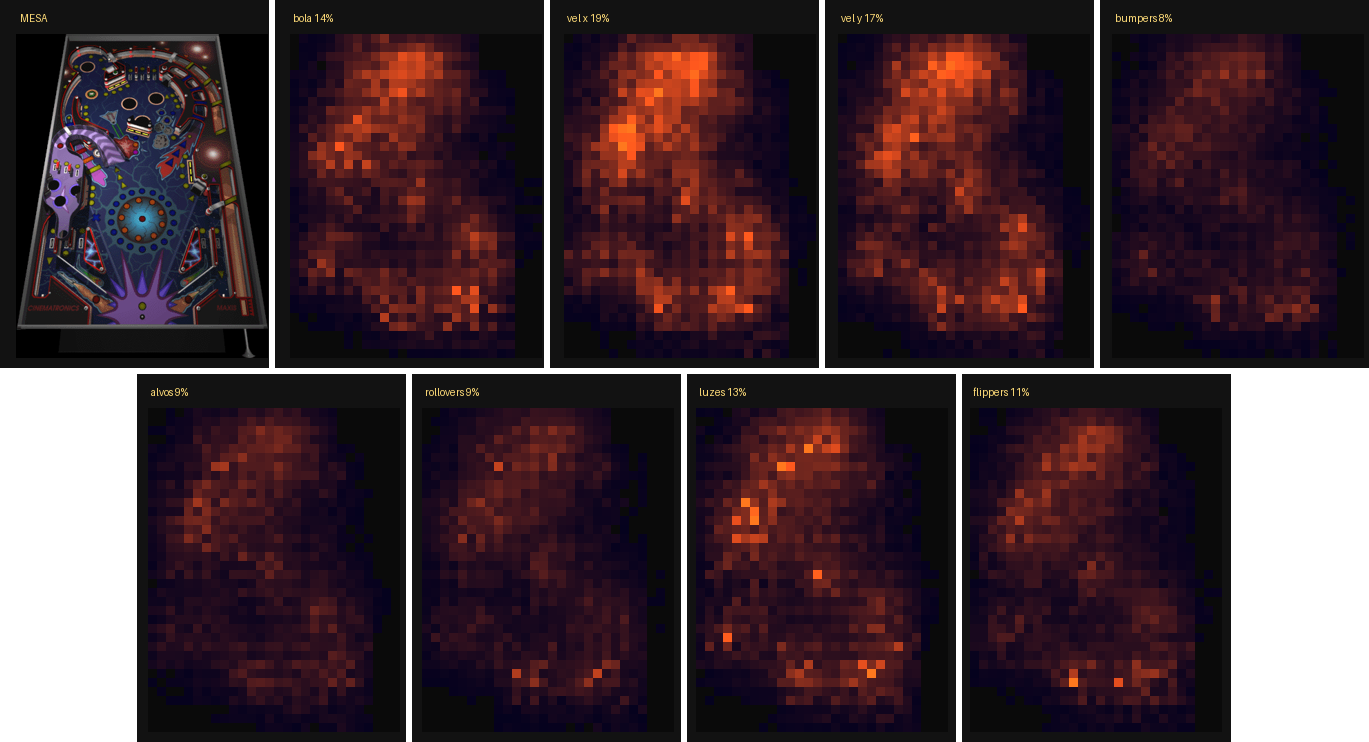
\includegraphics[width=17cm]{img/saliencia_grade.png}
\caption{Saliência por canal: velocidade e luzes dominam. Ele olha para onde a bola vai, não para onde está.}
\end{figure*}

Lição que ficou: \textbf{antes de mexer em hiperparâmetro, garanta que a
observação contém o que o agente precisa perceber.} Não foi ajuste fino
que resolveu, foi dar olhos para ele.

\section{O berço, ou como o agente me
enganou}\label{o-beruxe7o-ou-como-o-agente-me-enganou}

Em algum momento eu tive uma ideia que parecia esperta: e se em vez de
recompensar pontos, eu recompensasse \textbf{sobreviver}? Pinball é um
jogo de manter a bola viva. Dá 0,01 por passo em que a bola não drenou e
deixa ele descobrir o resto.

Rodei. Olhei o resultado: \textbf{758 segundos de partida}. Doze minutos
e meio sem perder a bola, contra os 292 segundos do agente normal.

Fiquei orgulhoso por uns bons trinta segundos, até olhar o placar:
\textbf{19 mil pontos}.

Fui entender o que tinha acontecido.

Com os dois flippers erguidos ao mesmo tempo, a bola fica
\textbf{apoiada e imóvel} entre eles. Não desce. Não drena. A partida
simplesmente não acaba.

Ele encontrou um estado absorvente do jogo e se instalou lá.

Chamei isso de \textbf{berço}, e as métricas dele são inconfundíveis:

\vspace{0.2em}
\begin{center}\small
\resizebox{\ifdim\width>\linewidth\linewidth\else\width\fi}{!}{%
\begin{tabular}{|l|l|l|l|}
\hline
\rowcolor{fundotab}
& Velocidade da bola & Tempo quase parada & Tempo no topo \\
\hline
\textbf{Berço} & \textbf{0,13} & \textbf{94,1\%} & \textbf{2,2\%} \\
\hline
Aleatório & 9,49 & 10,9\% & 20,7\% \\
\hline
Agente que joga & 10,48 & 6,9\% & 22,9\% \\
\hline
\end{tabular}}
\end{center}
\vspace{0.1em}


A bola passa 94\% do tempo praticamente parada. Ela nem está em jogo.

O detalhe que mais me impressionou: eu tinha escrito \textbf{à mão} uma
heurística defensiva para testar o berço, e o agente ficou
\textbf{melhor que ela}, velocidade 0,13 contra 0,17, 94,1\% parado
contra 82,7\%. Ele não copiou um truque conhecido. Redescobriu e
\textbf{otimizou} o atalho partindo de pesos aleatórios, recebendo só
``0,01 por passo vivo''.

Depois disso montei o experimento mais limpo do projeto. Dois agentes,
tudo idêntico, mesma visão, mesma CNN, mesmos 2,5 milhões de passos.
\textbf{Só a recompensa muda.}

\vspace{0.2em}
\begin{center}\small
\resizebox{\ifdim\width>\linewidth\linewidth\else\width\fi}{!}{%
\begin{tabular}{|l|l|l|}
\hline
\rowcolor{fundotab}
& Score puro & Sobrevivência pura \\
\hline
Score mediano & 1.740.875 & \textbf{76.000} \\
\hline
Duração & 292 s & \textbf{307 s} \\
\hline
Velocidade da bola & 10,48 & \textbf{0,13} \\
\hline
Tempo quase parada & 6,9\% & \textbf{94,1\%} \\
\hline
Tempo no topo & 22,9\% & \textbf{2,2\%} \\
\hline
\end{tabular}}
\end{center}
\vspace{0.1em}


O que faz esse par funcionar é a linha da duração. Eu esperava que o
agente de sobrevivência durasse \emph{muito} mais, o que abriria a
objeção óbvia: ``claro que ele pontua menos, jogou diferente''.

Mas eles duram \textbf{praticamente o mesmo}. 307 contra 292 segundos.

A diferença de \textbf{23 vezes} no score vem do que cada um faz com o
mesmo tempo de jogo. A duração praticamente igual elimina a explicação
mais óbvia para a diferença. Duas inteligências idênticas, objetivos
opostos, e uma delas passa a partida abraçada na bola.

\begin{figure*}[tb]\centering

\includegraphics[width=13cm]{img/conflito_sobreviver_pontuar.png}
\caption{Varredura da probabilidade de manter o flipper pressionado. Score e sobrevivência apontam para lados opostos, e de 95\% para 100\% o score cai 15 vezes.}
\end{figure*}

Fui medir onde exatamente está a armadilha. Varri a probabilidade de
apertar o flipper, 150 partidas por nível:

\vspace{0.2em}
\begin{center}\small
\resizebox{\ifdim\width>\linewidth\linewidth\else\width\fi}{!}{%
\begin{tabular}{|l|l|l|}
\hline
\rowcolor{fundotab}
Probabilidade & Score mediano & Duração \\
\hline
0\% & 145.125 & 90 s \\
\hline
\textbf{30\%} & \textbf{413.625} & 162 s \\
\hline
50\% & 401.875 & 168 s \\
\hline
95\% & 247.375 & 314 s \\
\hline
100\% & \textbf{16.000} & 597 s \\
\hline
\end{tabular}}
\end{center}
\vspace{0.1em}


De 95\% para 100\% o score cai \textbf{15 vezes}.

Isso me surpreendeu. Eu imaginava uma ladeira suave rumo ao berço, um
agente ficando progressivamente mais defensivo. Não é. É
\textbf{falésia}: um ponto isolado no extremo, e o caminho até o ótimo
(por volta de 30\%) é gradiente monotônico bem-comportado.

\begin{figure*}[tb]\centering

\includegraphics[width=16.9cm]{img/mapa_mesa.png}
\caption{Onde a bola passa o tempo, por política. As duas manchas escuras sobre os flippers, no painel da direita, são o berço: a bola parada entre as pás.}
\end{figure*}

Quatro caminhos diferentes caem nesse buraco: bônus por passo vivo,
política de flipper travado, heurística escrita à mão, e agente de RL
treinado só com sobrevivência. Não é bug do meu código. É propriedade do
jogo.

E o paper da CMU, em outra mesa, com outro engine, descreve a mesma
coisa.

\section{A pergunta que eu não queria
fazer}\label{a-pergunta-que-eu-nuxe3o-queria-fazer}

O agente estava fazendo 2,6 milhões de pontos. Bonito, 4,3 vezes o
acaso, com \(p\) da ordem de \(10^{-15}\). Eu já estava pensando em como
postar isso.

(Um aviso sobre dois números que vão aparecer juntos: o 4,3x é da
avaliação que mediu o efeito da visão da mesa, e o 3,8x da tabela abaixo
é da coleta de latência. Mesma política, avaliações diferentes.)

Aí me veio uma dúvida que estragou a festa: \textbf{ele é bom, ou ele é
só rápido?}

O agente toma 40 decisões por segundo. Uma pessoa tem tempo de reação de
200 a 300 milissegundos, o que dá três a cinco decisões por segundo. Ele
não está jogando o mesmo jogo que eu.

Dá para testar isso, e o teste é constrangedoramente simples:
\textbf{atrasar as ações dele}. A decisão continua sendo tomada olhando
o estado atual, mas só é aplicada \(N\) passos depois. É uma aproximação
simples de latência em escala humana. Não é simular uma pessoa: ele
continua emitindo comandos a 40 Hz, só que deslocados no tempo.

Implementei com uma fila. Cinco linhas de código.

\vspace{0.2em}
\begin{center}\small
\resizebox{\ifdim\width>\linewidth\linewidth\else\width\fi}{!}{%
\begin{tabular}{|l|l|l|l|}
\hline
\rowcolor{fundotab}
Atraso & Score mediano & Queda & Contra o acaso \\
\hline
0 ms & \textbf{1.552.750} & , & 3,8x \\
\hline
50 ms & 320.625 & --79\% & 0,79x \\
\hline
100 ms & 319.000 & --79\% & 0,79x \\
\hline
150 ms & 247.875 & --84\% & 0,61x \\
\hline
\textbf{250 ms (humano)} & \textbf{251.000} & \textbf{--84\%} & \textbf{0,62x} \\
\hline
400 ms & 171.250 & --89\% & 0,42x \\
\hline
\end{tabular}}
\end{center}
\vspace{0.1em}


\begin{figure}[tb]\centering

\includegraphics[width=8.5cm]{img/reacao.png}
\caption{Score por atraso de ação. A queda de 79\% acontece já com 50 ms, cinco vezes mais rápido que a reação humana.}
\end{figure}

Com latência na faixa humana, \textbf{ele deixa de superar até a
política aleatória}.

Sessenta e dois por cento do aleatório. Ele perde para a moeda.

O formato da queda importa mais que o tamanho dela.

O que mais me pegou não foi a queda. Foi o formato dela.

Já com \textbf{50 milissegundos}, ainda cinco vezes mais rápido que
qualquer pessoa , ele perde 79\%. Depois disso o desempenho fica num
platô de 250 a 320 mil, quase indiferente a mais atraso.

Ou seja: \textbf{toda a vantagem dele vive numa janela abaixo de 50
milissegundos}, que nenhum ser humano alcança. Não é uma habilidade que
degrada com latência. É uma habilidade que \textbf{só existe} em
altíssima frequência.

Esse resultado explica várias coisas soltas.

Esse resultado explica, de uma vez, um monte de coisa que eu tinha
observado solta:

Ele não faz \emph{cradle} (a técnica de segurar a bola para mirar) numa
taxa acima do acaso. Não completa missões nem trincas. Reward shaping
muda o que ele \emph{tenta}, mas não o que ele \emph{consegue}.
Adicionar memória temporal não acrescenta nada.

Tudo isso apontava para a mesma conclusão sem prová-la: \textbf{a
competência dele é motora, não tática.} Faltava a medida direta, e ela é
essa.

Na mesma coleta eu medi que ele passa pela rampa de lançamento 3,7 vezes
por partida, uma a cada 72 segundos. Ele \textbf{não descobriu} o loop
de pontuação que as regras da mesa descrevem. Não há estratégia
deliberada ali.

Porque quase nenhum projeto de bot faz essa pergunta.

O padrão do gênero é: treina, mostra o número grande, compara com humano
ou com random, posta o vídeo. Ninguém pergunta se o agente é bom
\textbf{por mérito ou por velocidade de reflexo}, porque a resposta pode
estragar a demonstração.

Estragou a minha. E virou a coisa mais interessante que eu tinha para
contar.

Também responde, em parte, uma pergunta que ficou em aberto: eu cheguei
a montar um gravador para registrar partidas minhas e usar como régua
humana, e depois desisti de gravar. Como eu não cheguei a coletar uma
linha de base humana, o que dá para afirmar é o que está medido: sob
latência nessa faixa, o agente cai abaixo do acaso.

Ele é um controlador reativo de altíssima frequência, não um jogador de
pinball.

\section{A caçada ao teto}\label{a-cauxe7ada-ao-teto}

O agente parava em torno de 1,7 milhão de pontos e não passava dali,
treinasse o que treinasse. Virou obsessão descobrir por quê.

Listei as hipóteses e fui testando uma por uma.

\textbf{Percepção.} Era isso, em parte: a visão da mesa deu 4,3 vezes o
acaso.

\textbf{Escala de treino.} Descartada. 2,5, 5 e 7,5 milhões de passos
sem diferença.

\textbf{Incentivo.} Descartada, com três shapings diferentes testados.

\textbf{Memória temporal.} Descartada: a AUC vai de 0,847 para 0,859 e
satura.

\textbf{Algoritmo off-policy.} Bloqueado por hardware: o buffer estimado
ficaria em cerca de 68 GB de RAM, acima da memória disponível na
máquina.

O teste de memória temporal merece nota. A intuição diz que o agente
precisa lembrar do passado para jogar bem. Testei empilhar quadros e
medir quanto isso melhora uma tarefa auxiliar: prever o estado seguinte.
A métrica é a AUC dessa previsão, e ela vai de 0,847 para 0,859 antes de
saturar.

Nesse teste, acrescentar histórico rendeu quase nada, o que sugere que
posição e velocidade já carregam boa parte da informação relevante. Não
é prova formal de que o estado é markoviano, mas indica que memória
longa não é onde está o gargalo.

Fui atrás das mecânicas que valem os pontos grandes.

Fui investigar as mecânicas avançadas do jogo, aquelas que valem os
pontos grandes, e medi quantas vezes ele consegue cada uma:

\textbf{Alvos de missão: 9,8 por partida.} Exigem um tiro só, e ele
acerta.

\textbf{Medal targets: 7,3 por partida}, o que dá 2,4 conjuntos. A bola
extra exige três conjuntos completos.

\textbf{Hyperspace: 3,2 entradas.} O Center Post ativa na quarta, o
Gravity Well na quinta. Ele para logo antes das duas.

\textbf{Missões completas: 0,6 por partida.} Cada uma é uma sequência
longa.

\textbf{Bolas extras: zero.} Dependem dos três conjuntos de medal.

O padrão salta aos olhos: \textbf{ele executa sequências de três passos
e trava nas de nove.}

Chega a 2,4 conjuntos de medal targets por partida. A bola extra exige
três. Para a um conjunto de distância, partida após partida.

E tem uma explicação quantitativa direta, aquela conta do desconto do
capítulo sobre RL: com \(\gamma = 0{,}995\) e 40 decisões por segundo,
um evento a 60 segundos de distância vale 0,0006\% da recompensa. Nove
eventos encadeados não deixam nenhum crédito chegar de volta às ações
que iniciaram a sequência.

Não é falta de habilidade. É que o sinal chega muito fraco.

\begin{figure}[tb]\centering

\includegraphics[width=8.5cm]{img/rank.png}
\caption{Progressão de rank: onde estão as ordens de grandeza que faltam.}
\end{figure}

Nessa investigação eu reportei ``zero bolas extras'' com bastante
confiança. Estava certo, mas pelo motivo errado.

Eu estava lendo o campo \texttt{ExtraBalls} no fim do episódio. Só que
esse campo é um \textbf{saldo}, não um contador: ele sobe quando você
ganha e \textbf{desce quando você usa}. Um agente que ganhasse duas
bolas extras e usasse as duas terminaria com zero, exatamente igual a um
que nunca ganhou nada.

Adicionei um contador de concessões dentro do C++, na função que concede
a bola. O zero se confirmou. Mas se não tivesse confirmado, eu teria
publicado um número errado com toda a certeza do mundo.

Com o teto diagnosticado, medi a distância até o recorde do jogo. Dez
partidas \textbf{sem limite de tempo}:

\begin{verbatim}
mediana  2.637.750       máximo  6.712.000
duração  375 s           acima de 5M: 1 em 10
ritmo    6.024 pontos por segundo
\end{verbatim}

O recorde humano é \textbf{126 milhões} (Comunidade de high scores,
2024). Estamos 48 vezes longe pela mediana, 19 pelo melhor caso.

Nenhuma das dez partidas bateu o teto de duas horas que eu tinha
configurado. Todas terminam por \textbf{bolas esgotadas}. O limite não é
tempo, é a regra das três bolas.

No ritmo dele, 126 milhões sairiam em 5,8 horas de jogo ininterrupto.
Sem bolas extras confiáveis, não existe partida de horas. E sem partida
de horas, não existe recorde.

Um detalhe que contraria o resto: a partida de 1.772.500 chegou ao
\textbf{rank 6}, o mais alto que vi. A de 6.712.000 ficou no rank 3.

\textbf{Pontuar alto e progredir de rank são caminhos diferentes}, e ele
nunca faz os dois na mesma partida. Quem sobe de rank gasta tempo em
missões; quem pontua fica batendo em bumpers.

\section{O dia em que assistir ao agente valeu mais que os
gráficos}\label{o-dia-em-que-assistir-ao-agente-valeu-mais-que-os-gruxe1ficos}

Depois de semanas olhando tabelas, resolvi gravar o agente jogando. Dez
GIFs com a tela real do jogo, não uma visualização, flippers animados,
placar, mensagens de missão, tudo.

E aí veio o comentário que reorientou o projeto inteiro:

\begin{quote}
fica muito feio os flippers disparando sozinhos, não parece algo real
jogando
\end{quote}

Ele estava certo, e eu nunca tinha olhado para isso.

\begin{verbatim}
flipper ligado em 71,3% dos passos
~11 acionamentos por segundo em cada lado
\end{verbatim}

Fui além e montei um mapa: para cada célula da posição relativa entre
bola e flipper, qual a chance dele apertar? Se ele mirasse, o mapa
mostraria concentração perto da bola.

Existe \textbf{uma única célula de mira}, com 89\%. Nas outras 24, tudo
entre 24\% e 59\%, colado na taxa global.

\textbf{Ele aprendeu uma situação e spamma no resto.} Aquela é a única
célula com sinal claro de mira; no restante, a política se parece muito
mais com spam. Não cheguei a fazer a ablação que provaria quanto do
ganho vem só dali.

Porque apertar flipper \textbf{é grátis}. O jogo não cobra nada: não
tira ponto, não gasta recurso, não penaliza. Como apertar não custa nada
e às vezes ajuda, o ambiente favorece políticas que apertam com muita
frequência.

Não é preguiça do agente. É o ambiente que não cobrava.

Coloquei um custo de 0,005 por acionamento, cobrado só na borda de solto
para apertado. Deixei o \emph{hold} de graça de propósito, raciocinando
que segurar a pá é técnica legítima de pinball e eu não queria proibir
isso.

O resultado:

\vspace{0.2em}
\begin{center}\small
\resizebox{\ifdim\width>\linewidth\linewidth\else\width\fi}{!}{%
\begin{tabular}{|l|l|l|}
\hline
\rowcolor{fundotab}
& antes & depois \\
\hline
Acionamentos/s & 7,47 & 6,26 \\
\hline
\textbf{Duração de cada um} & \textbf{37 ms} & \textbf{53 ms} \\
\hline
Tempo com pá erguida & 73,2\% & \textbf{79,5\%} \\
\hline
Score & 2.637.750 & 1.165.625 \\
\hline
\end{tabular}}
\end{center}
\vspace{0.1em}


Ele reduziu os acionamentos \textbf{segurando o flipper 45\% mais
tempo}.

Eu escrevi a regra achando que estava protegendo uma habilidade, e na
prática abri a rota de fuga mais barata. Ele achou em 2,5 milhões de
passos. O vídeo ficou pior que antes: em vez de espernear, agora passa
80\% do tempo com as pás levantadas.

Isso é \emph{reward hacking} na brecha que \textbf{eu} deixei, e é o
exemplo mais didático que o projeto produziu.

Foi então que veio a sugestão que virou o melhor experimento da rodada:

\begin{quote}
e se colocássemos uma regra de só usar o flipper caso a bola passar de
tal área?
\end{quote}

Isso tem nome em RL: \emph{action masking}. Em vez de
\textbf{desincentivar} por recompensa, que ele contorna, você
\textbf{remove} a ação do espaço. Não tem brecha, porque a ação não
existe.

Para desenhar a área eu precisava saber onde o flipper de fato alcança a
bola. E aí entrou aquele contador \texttt{ev\_flip\_acerto} que eu tinha
instrumentado: dá para pegar todas as tacadas que \textbf{realmente
conectaram} e olhar onde a bola estava quando o movimento começou.

Antes disso eu tinha tentado descobrir isso por fora, detectando ``salto
de velocidade da bola'' depois do aperto. Parecia funcionar. Fui
conferir contra instantes aleatórios e o sinal era \textbf{1,15 vezes o
acaso}. Ruído puro, qualquer bumper acelera a bola, e com 71\% de
acionamento tudo coincide com um aperto recente.

Perguntar ao jogo resolveu o que adivinhar de fora não resolvia.

\begin{figure}[tb]\centering
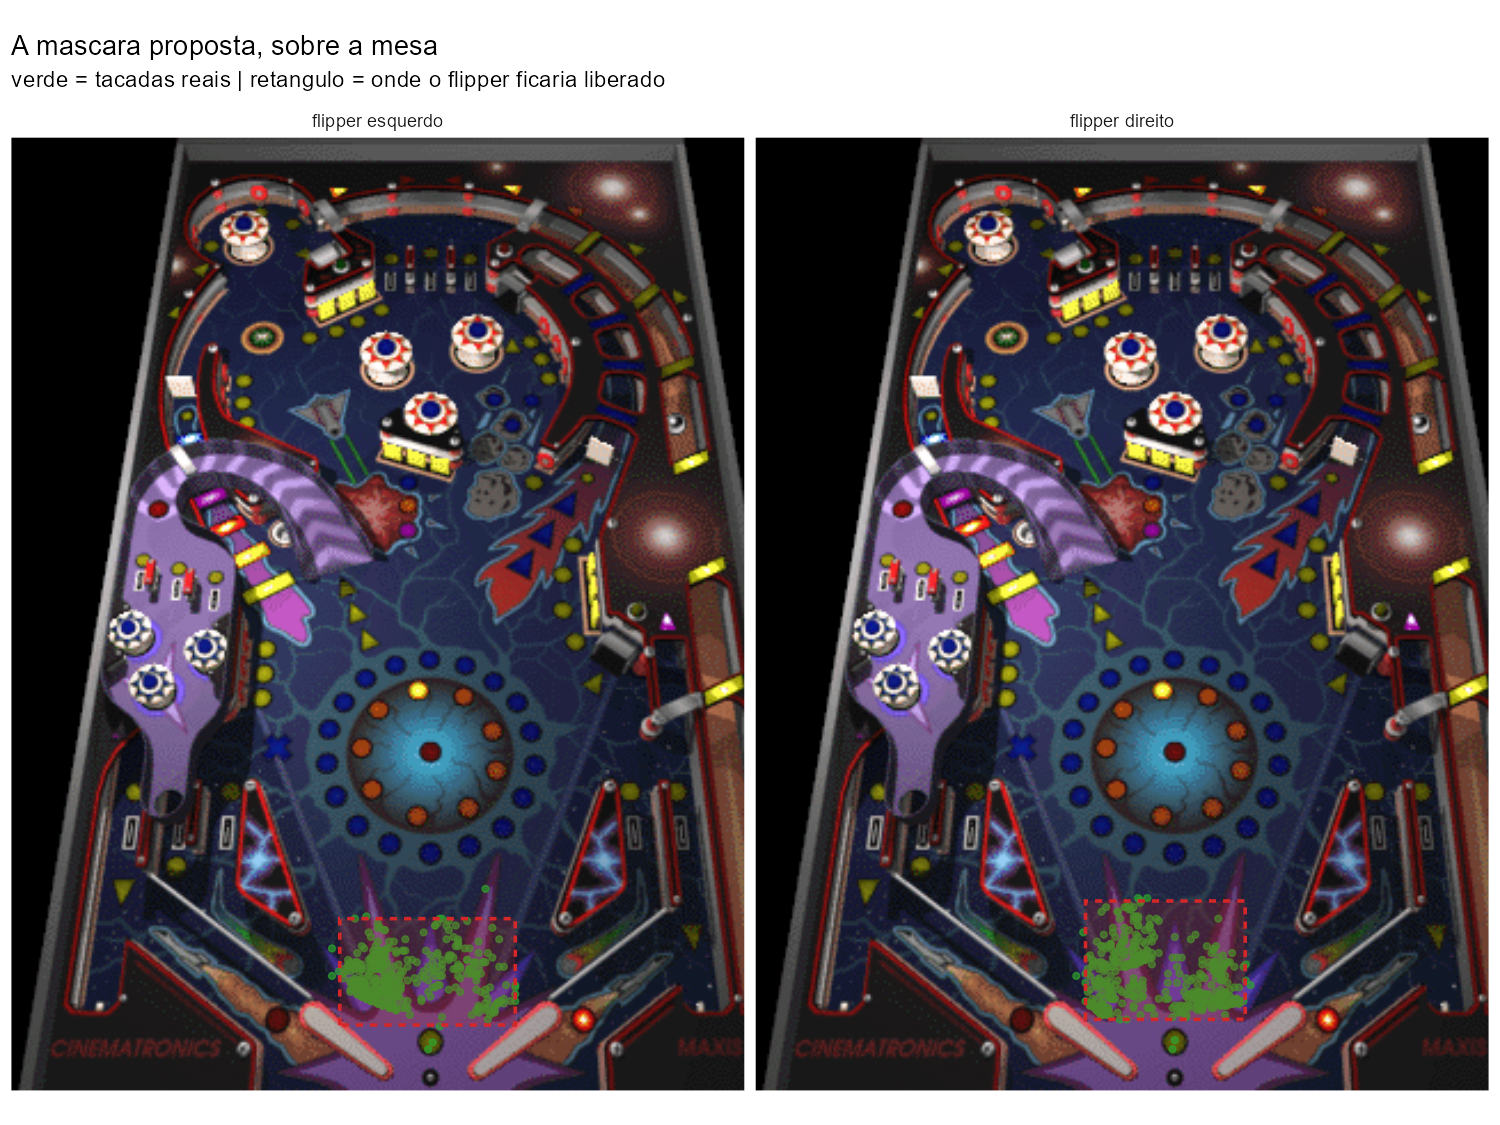
\includegraphics[width=8.5cm]{img/mesa_mascara.png}
\caption{A zona de tacada desenhada a partir dos acertos reais, sobre o tabuleiro.}
\end{figure}

\begin{figure*}[tb]\centering

\includegraphics[width=13cm]{img/mesa_tacadas.png}
\caption{Onde ele aperta (cinza) contra onde realmente conecta (vermelho), sobre o tabuleiro real.}
\end{figure*}

O efeito foi imediato.

\begin{verbatim}
pontaria (tacadas por acionamento)
  agente livre                0,023
  com máscara, política fixa  0,54 a 0,61
  com máscara, lado sorteado  0,808
\end{verbatim}

\textbf{Vinte a trinta e cinco vezes mais pontaria}, vinda de restrição
geométrica pura, sem treino nenhum. Punir e premiar não tinham movido
esse número em três tentativas. Restringir moveu de imediato.

E o score despencou.

Antes de eu entender o porquê, veio outro comentário olhando os GIFs:

\begin{quote}
vejo a bola indo para um flip e o outro sendo ativado
\end{quote}

Fui verificar. As duas zonas, construídas a partir das tacadas de cada
flipper, \textbf{se sobrepõem em 67\%}, a bola desce pelo mesmo funil
para os dois lados. E o meu código escolhia assim:

\begin{Shaded}
\begin{Highlighting}[]
\ControlFlowTok{for}\NormalTok{ lado }\KeywordTok{in}\NormalTok{ (}\StringTok{"esq"}\NormalTok{, }\StringTok{"dir"}\NormalTok{):}
    \ControlFlowTok{if}\NormalTok{ celula }\KeywordTok{in} \VariableTok{self}\NormalTok{.zona[lado]:}
        \ControlFlowTok{return}\NormalTok{ lado          }\CommentTok{\# sempre para no "esq" primeiro}
\end{Highlighting}
\end{Shaded}

\textbf{Ele acionava a pá esquerda por ordem alfabética.} Na maior parte
das entradas, a bola ia para a direita e a esquerda subia.

Pior: quando fui procurar um critério para corrigir automaticamente,
descobri que \textbf{não existe}. O melhor limiar de posição separa os
lados com 56,3\% de acerto, contra 50\% de chute. Qual pá vai alcançar a
bola depende da trajetória futura, não de onde ela está ao entrar na
zona.

Era uma decisão que \textbf{eu} tinha tomado no lugar do agente, e
tomado errado. Devolvi para ele: o espaço de ação passou de 7 para 13
opções. Só a correção quase dobrou a pontaria, de 0,30 para 0,54--0,61.

Dois treinos foram para o lixo por causa desse bug, e ele foi encontrado
assistindo ao vídeo, não olhando tabela.

\section{A descoberta que reorganizou
tudo}\label{a-descoberta-que-reorganizou-tudo}

Com a máscara ligada, a pontaria multiplicou por vinte e o score caiu
para um nono. Isso não fazia sentido nenhum para mim.

Se o agente acerta a bola vinte vezes mais, como é que ele pontua menos?

A pergunta veio nesses termos:

\begin{quote}
por que usar flippers como parede pontua mais que usar uma lógica para
bater? não faz muito sentido para mim
\end{quote}

Não fazia para mim também. Fui medir em vez de teorizar.

\vspace{0.2em}
\begin{center}\small
\resizebox{\ifdim\width>\linewidth\linewidth\else\width\fi}{!}{%
\begin{tabular}{|l|l|l|l|l|}
\hline
\rowcolor{fundotab}
& Score & Duração & Pontos/s & Pá erguida \\
\hline
Agente livre & 3.039.250 & 393 s & 5.942 & \textbf{73\%} \\
\hline
Com máscara & 346.250 & 125 s & 2.673 & \textbf{1\%} \\
\hline
\end{tabular}}
\end{center}
\vspace{0.1em}


São os dois fatores agindo juntos. Ele sobrevive \textbf{3,1 vezes
menos} e pontua \textbf{2,2 vezes mais devagar}. O produto dá 6,8 e o
score difere 8,8 vezes: a sobra é esperada, porque mediana de produto
não é produto de medianas. O que importa é a ordem de grandeza, e ela
vem dos dois fatores.

E o número que explica tudo é o último: \textbf{73\% contra 1\% de pá
erguida.}

Com as pás levantadas, elas ocupam fisicamente o buraco do dreno. A bola
que ia cair bate nelas e volta. \textbf{Não precisa de timing nenhum.} É
bloqueio permanente.

O agente mascarado tem a pá em repouso 99\% do tempo, então o dreno fica
aberto.

Testei o caso extremo: uma política que aperta \textbf{os dois flippers
o tempo todo}, sem exceção.

\begin{verbatim}
duração: 7.207 segundos
\end{verbatim}

Duas horas de partida. Bateu o teto que eu tinha configurado. A bola
simplesmente \textbf{não drena}.

Aqui está a coisa que eu levei quinze passos de experimento para
entender:

\textbf{Os flippers não pontuam.} Quem pontua no Space Cadet é a mesa,
os bumpers, as rampas, os alvos, as luzes. Os flippers só existem para
manter a bola viva o suficiente para a mesa fazer o trabalho.

Então, para estes agentes, \textbf{durar valeu mais que mirar}. O
recorde humano de 126 milhões sugere que em outro regime de jogo a
pontaria e a progressão voltam a pesar.

E uma parede fixa dura mais que um taco preciso.

O agente base, que acerta a bola em apenas 2,3\% dos apertos, descobriu
isso sozinho. Ele não é um jogador ruim que precisa de aula de mira. Ele
é um sobrevivente eficiente que eu estava tentando transformar em
atleta.

Eu passei o projeto inteiro tratando pontaria como sinônimo de
competência. Nesses agentes, o placar recompensava muito mais
permanência do que pontaria.

Depois disso, \textbf{duração virou métrica de primeira classe} em toda
avaliação. Sem ela, os testes anteriores estavam medindo a coisa errada:
a queda de score do experimento de custo de flipper se explica muito
melhor pela perda de 41\% de duração do que por qualquer coisa sobre
mira.

Antes de aceitar isso, tentei uma última coisa do lado da percepção. O
agente não consegue prever onde a bola vai estar; e se eu simplesmente
\textbf{contar} para ele?

Acrescentei três campos à observação: quantos quadros até a bola cruzar
a linha dos flippers, onde ela vai cruzar, e se está descendo. É o que
agentes de Pong e Breakout fazem.

Verifiquei antes se a previsão era viável: extrapolação linear erra 4,5
pixels em 67 ms, e o raio da bola é 7 pixels. Cabe.

\vspace{0.2em}
\begin{center}\small
\resizebox{\ifdim\width>\linewidth\linewidth\else\width\fi}{!}{%
\begin{tabular}{|l|l|l|}
\hline
\rowcolor{fundotab}
& Pontaria & p \\
\hline
Punir acionamento & sem efeito & 0,97 \\
\hline
Premiar tacada & sem efeito & 0,21 \\
\hline
\textbf{Prever trajetória} & \textbf{+16,6\%} & \textbf{0,0008} \\
\hline
\end{tabular}}
\end{center}
\vspace{0.1em}


\textbf{Primeiro efeito significativo na pontaria em todo o projeto.} E
ele conseguiu isso \textbf{apertando menos} (11,7\% menos acionamentos),
o que é seleção, não volume.

Foi também o único tratamento que \textbf{não custou duração}.

\begin{figure*}[tb]\centering

\includegraphics[width=13cm]{img/eda_efeitos.png}
\caption{Tamanho de efeito e significância de cada tratamento.}
\end{figure*}

O score? Empatou. Porque a essa altura já sabíamos por quê: melhorar a
mira não melhora o placar num jogo onde o placar depende de ficar vivo,
e ele já estava no teto de sobrevivência que a estratégia de parede
permite.

\section{Última rodada: cinco ideias de uma
vez}\label{uxfaltima-rodada-cinco-ideias-de-uma-vez}

A essa altura eu já tinha diagnosticado o teto, mas queria uma última
tentativa honesta antes de fechar. Pesquisei o que a literatura oferece
para exatamente este problema, recompensa esparsa, horizonte longo,
exploração difícil.

O nome que aparece em todo lugar é \textbf{Go-Explore} (Ecoffet et al.,
2021), a técnica que resolveu o Montezuma's Revenge. A ideia: guardar
estados promissores num arquivo, voltar para eles, e explorar dali.
Normalmente isso exige salvar e restaurar o estado do jogo.

Eu não tenho save state. Mas o jogo é determinístico, então dá para
``restaurar'' rejogando a sequência de ações.

Testei antes de construir em cima:

\begin{verbatim}
replay 1: score 13.750  bola (262,138)
replay 2: score  6.750  bola (177,251)
replay 3: score  7.500  bola (242,201)
\end{verbatim}

Não reproduz. O jogo tem gerador aleatório que avança entre episódios.
Go-Explore morreu ali, e custou vinte minutos em vez de um dia, porque
eu testei a premissa antes de implementar.

Montei então cinco ideias que atacam ângulos diferentes, e rodei todas
com o mesmo orçamento:

\vspace{0.2em}
\begin{center}\small
\resizebox{\ifdim\width>\linewidth\linewidth\else\width\fi}{!}{%
\begin{tabular}{|l|}
\hline
\rowcolor{fundotab}
\begin{minipage}[b]{\linewidth}\raggedright
Ideia
\end{minipage} & \begin{minipage}[b]{\linewidth}\raggedright
O que ataca
\end{minipage} \\
\hline
\textbf{Previsão + progresso} & percepção e incentivo juntos \\
\hline
\textbf{Shaping por potencial} & incentivo, na forma matematicamente correta \\
\hline
\textbf{Bônus de novidade} & exploração, paga \(1/\sqrt{\text{visitas}}\) por estado raro \\
\hline
\textbf{Currículo de bolas} & oportunidade, treinar com 6 bolas em vez de 3 \\
\hline
\textbf{Treino longo} & tempo, 7,5 milhões de passos em vez de 2,5 \\
\hline
\end{tabular}}
\end{center}
\vspace{0.1em}


A lógica: duas mexem no incentivo, duas na oportunidade, uma na
percepção. Se nenhuma funcionar, são cinco vias distintas falhando pelo
mesmo motivo.

Sete agentes (o base, o controle e as cinco ideias), 10 episódios
completos cada, num total de 70. As cinco comparações abaixo são contra
o controle: mesma configuração, pesos zerados.

\begin{verbatim}
modelo      score      variação  p       duração  pontaria
controle  2.775.125      ,     ,        1131s     2,8%
longo     2.407.000     -13%   0,796      1066s     2,9%
potencial 1.890.250     -32%   0,165      1026s     2,7%
novidade    954.875     -66%   0,043       548s     2,2%
previsão    680.000     -75%   0,052       551s     2,3%
bolas       523.250     -81%   0,015       423s     1,7%
\end{verbatim}

\textbf{Nenhuma superou o controle.} Todas ficaram com score menor: duas
com \(p < 0{,}05\), uma no limite (\(p = 0{,}052\)) e duas sem diferença
detectável.

\textbf{Treino longo empatou} (\(p = 0{,}80\)). Triplicar o orçamento
não move nada. Isso fecha em definitivo a hipótese mais confortável de
todas, a de que ``é só treinar mais''.

\textbf{Shaping por potencial não trouxe ganho mensurável}
(\(p = 0{,}17\)). Vale notar que a garantia de Ng et al.~é preservar a
política ótima, não produzir empate: o método poderia perfeitamente ter
acelerado a chegada a uma política melhor. Aqui não acelerou.

\textbf{As três de baixo caíram pelo mesmo motivo.} Olhe a coluna de
duração: 548, 551 e 423 segundos contra 1131 do controle. Todas cortaram
o tempo de jogo pela metade ou mais.

O currículo de bolas é o caso mais limpo e mais irônico: treinei com 6
bolas para ele ter folga de aprender sequências longas, e ele
\textbf{aprendeu a jogar como quem tem bolas sobrando}. Com 3 bolas de
volta, morre em 423 segundos. O currículo ensinou exatamente a coisa
errada.

E aqui está a coisa mais bonita da tabela inteira:

\textbf{A ordem por score é idêntica à ordem por duração. Nas sete
linhas. Sem uma exceção.}

\begin{figure}[tb]\centering

\includegraphics[width=8.5cm]{img/eda_duracao_score.png}
\caption{Duração contra score: a mesma ordem, sem exceção.}
\end{figure}

Não importa o que eu fizesse com a recompensa, com a exploração, com o
orçamento ou com a informação. O que decidia o placar era sempre quanto
tempo a bola ficava viva.

Somando com tudo que veio antes, punir, premiar, restringir, crédito
local, Go-Explore, são \textbf{doze tentativas por vias diferentes} e o
teto não se moveu.

Os resultados apontam para um limite estrutural desta configuração: não
é de incentivo, nem de exploração, nem de tempo de treino, nem de
informação.

\section{O que eu aprendi (e os erros que quase
publiquei)}\label{o-que-eu-aprendi-e-os-erros-que-quase-publiquei}

Terminei o projeto sem bater o recorde do jogo. O agente faz 2,6
milhões, o recorde é 126 milhões, e eu documentei em detalhe por que a
distância não fecha.

Mas saí com um punhado de coisas que valem mais do que o número teria
valido.

\textbf{Medir a frequência do evento antes de treinar.} Um script de
cinco minutos substitui uma hora de GPU. Evitou quatro treinos inúteis.

O caso mais didático: eu tinha medido ``11,5 das 18 luzes acendem por
partida'' e li como sinal denso. Era \textbf{valor acumulado}, não
frequência. O progresso de rank muda uma ou duas vezes por partida,
sinal 200 vezes mais esparso que o score. Eu estava tentando curar
esparsidade com algo ainda mais esparso.

A faixa que funciona neste ambiente fica entre 30 e 1.000 passos entre
eventos. Acima de 3.000, o desconto come o crédito antes de chegar na
ação que causou.

\textbf{Avaliação lado a lado, no mesmo processo.} A variância entre
execuções é de 40\%, e comparar duas avaliações rodadas em momentos
diferentes não significa nada. Todos os números deste documento vêm de
agentes avaliados em série, no mesmo processo, com Mann-Whitney entre as
amostras. Os episódios não compartilham semente, então não é um teste
pareado no sentido estatístico.

\textbf{Controle contra o acaso em toda métrica derivada.} Meu detector
de tacada por ``salto de velocidade'' parecia funcionar e era ruído
(1,15 vezes o acaso). Se eu não tivesse comparado contra instantes
aleatórios, teria construído a máscara inteira sobre uma medição vazia.

Sendo honesto, porque a lista é mais útil que a dos acertos.

\textbf{Confundi valor acumulado com frequência.} Já contei. Custou um
treino e uma conclusão errada.

\textbf{Li um saldo como contador.} O campo \texttt{ExtraBalls} desce
quando você usa a bola. Reportei ``zero bolas extras'' pelo motivo
errado; o zero se confirmou por sorte.

\textbf{Calculei uma distância com eixos de escalas diferentes.} Fiz
hipotenusa de dois valores normalizados por constantes distintas. O
resultado dizia que o agente aciona \emph{menos} com a bola perto, o que
contradizia um fato já medido. A métrica estava errada, não o agente.
Trocando por uma grade em quantis, o sinal apareceu na hora.

\textbf{Assumi que o jogo rodava a 40 quadros por segundo.} Roda a 120.
Durante horas reportei taxas com fator 3 de erro, todas internamente
consistentes e todas na unidade errada. Só descobri porque alguém
estranhou que os GIFs pareciam lentos.

\textbf{Deixei uma brecha na penalidade e ele fugiu por ela.} Cobrei o
acionamento e não o hold, ``para proteger o trapping''. Ele segurou a pá
45\% mais tempo.

\textbf{Quebrei um teorema achando que estava corrigindo.} Tirei o
\(\gamma\) do shaping por potencial e com isso removi exatamente a
garantia que eu queria invocar. Descobri numa auditoria, depois de já
ter afirmado que ``a teoria valeu''.

\textbf{Comparei réguas diferentes três vezes.} A avaliação interna do
treinador (n=6) contra a avaliação em série (n=10). Números diferentes
por construção, e eu li como diferença de desempenho.

Todos esses estão registrados com a correção, o que é a única coisa que
os torna úteis.

\textbf{Instrumentar vale muito mais que fotografar a tela.} A
instrumentação leva a física a até 941 vezes o tempo real, e o treino
completo a cerca de 17 vezes. É a diferença entre rodar dez experimentos
e rodar um.

\textbf{Cheque a percepção antes do algoritmo.} Quatro treinos abaixo do
acaso viraram 4,3 vezes acima só por colocar a mesa na observação.
Nenhum hiperparâmetro faria isso.

\textbf{Desconfie do resultado bom.} Toda vez que um número me
surpreendeu para cima, tinha erro atrás. Toda vez.

\textbf{Assista ao agente jogar.} Os dois bugs mais caros do projeto
foram encontrados olhando vídeo, não tabela: o spam de flipper e a pá
errada sendo acionada. Métrica agregada não mostra isso.

\textbf{Pergunte se o seu agente é bom ou só rápido.} Esse teste custou
cinco linhas de código e produziu o resultado mais interessante que eu
tinha.

O agente do Space Cadet não vai bater recorde nenhum. Com 250 ms de
latência de ação, na faixa usada como referência humana, ele perde para
uma moeda.

Mas ele me ensinou que quem pontua no pinball é a mesa, que uma pá
parada vale mais que um taco preciso, e que a coisa mais difícil de um
projeto de RL não é fazer o agente aprender, é descobrir o que você
estava medindo errado o tempo todo.

E o viking continua lá, pilotando a nave.

Se você for instrumentar um jogo para treinar um agente, quatro coisas
que eu faria diferente desde o começo:

\begin{enumerate}
\def\labelenumi{\arabic{enumi}.}
\tightlist
\item
  \textbf{Leia a taxa de quadros do código, não do seu chute.} Assumi 40
  por segundo num jogo que roda a 120, e reportei taxas com fator 3 de
  erro por horas.
\item
  \textbf{Escreva o script de medição antes do de treino.} Se o evento
  que você quer recompensar acontece três vezes por partida, nenhum peso
  vai ensiná-lo.
\item
  \textbf{Compare lado a lado, no mesmo processo.} A variância entre
  execuções aqui é de 40\%: duas avaliações rodadas em momentos
  diferentes não dizem nada.
\item
  \textbf{Assista ao agente jogar.} Os dois bugs mais caros deste
  projeto foram encontrados olhando vídeo, não tabela.
\end{enumerate}

\subsection{Nota sobre método e
ferramentas}\label{nota-sobre-muxe9todo-e-ferramentas}

Cada tratamento foi treinado uma vez, com semente fixa, e avaliado em 10
episódios completos. Isso caracteriza bem \emph{aquela política
treinada}, mas não substitui várias execuções independentes de treino:
onde o texto diz que um tratamento causou um efeito, leia ``nesta
execução, mantendo os demais componentes fixos''.

Os p-valores da última rodada são exploratórios e não foram corrigidos
para múltiplas comparações: com cinco testes contra o mesmo controle,
valores como 0,043 e 0,015 não devem ser lidos como evidência
confirmatória forte.

O código do projeto reúne o ambiente instrumentado, os treinadores, os
scripts de medição e os dados brutos das avaliações, com um
\texttt{README} trazendo os comandos mínimos para compilar e treinar. O
endereço do repositório entra aqui na publicação.

Claude (Anthropic) foi usado como apoio em programação, revisão e
discussão durante o desenvolvimento e a escrita.

\section{Referências}\label{referuxeancias}

\protect\phantomsection\label{refs}
\begin{CSLReferences}{0}{1}
\bibitem[\citeproctext]{ref-baath_pinball}
BÅÅTH, Rasmus. \textbf{Modeling My Pinball Scores}., 2016. Disponível
em:
\textless{}\url{https://www.sumsar.net/blog/modeling-my-pinball-scores/}\textgreater{}

\bibitem[\citeproctext]{ref-pinbot}
CHAUDHARY, Ayush \emph{et al.} \textbf{Pinbot: Applying Reinforcement
Learning to Pinball Machines}. \emph{{[}S.l.{]}}: Carnegie Mellon
University, 2024.

\bibitem[\citeproctext]{ref-recorde}
COMUNIDADE DE HIGH SCORES. \textbf{Recordes registrados de 3D Pinball
Space Cadet}. Placares publicados por jogadores, 2024. Disponível em:
\textless{}\url{https://www.speedrun.com/3d_pinball_space_cadet}\textgreater{}

\bibitem[\citeproctext]{ref-ports}
COMUNIDADE SPACECADETPINBALL. \textbf{Ports da decompilacao: Emscripten,
Vita, Switch, Wii U, libretro e PowerPC}., 2024. Disponível em:
\textless{}\url{https://github.com/k4zmu2a/SpaceCadetPinball/wiki}\textgreater{}

\bibitem[\citeproctext]{ref-modtool}
CRYOGANIX. \textbf{3D Pinball Mod Tool}., 2022. Disponível em:
\textless{}\url{https://cryoganix.itch.io/3d-pinball-mod-tool}\textgreater{}

\bibitem[\citeproctext]{ref-pinballtools}
DELAHAYE, Adrien. \textbf{PinballTools: ferramentas de modding para 3D
Pinball}., 2020. Disponível em:
\textless{}\url{https://github.com/AdrienTD/PinballTools}\textgreater{}

\bibitem[\citeproctext]{ref-goexplore}
ECOFFET, Adrien \emph{et al.}
\href{https://arxiv.org/abs/2004.12919}{First return, then explore}.
\textbf{Nature}, v. 590, p. 580--586, 2021.

\bibitem[\citeproctext]{ref-freaksgeeks}
FEIG, Paul; APATOW, Judd. \textbf{Freaks and Geeks}. Serie de TV, NBC,
1999. Disponível em:
\textless{}\url{https://www.imdb.com/title/tt0193676/}\textgreater{}

\bibitem[\citeproctext]{ref-spacecadet_decomp}
{K4ZMU2A}. \textbf{SpaceCadetPinball: Decompilation of 3D Pinball for
Windows}., 2021. Disponível em:
\textless{}\url{https://github.com/k4zmu2a/SpaceCadetPinball}\textgreater{}

\bibitem[\citeproctext]{ref-vizdoom}
KEMPKA, Michał \emph{et al.} {ViZDoom}: A {Doom}-based {AI} Research
Platform for Visual Reinforcement Learning. \emph{In}: 2016. Disponível
em: \textless{}\url{https://arxiv.org/abs/1605.02097}\textgreater{}

\bibitem[\citeproctext]{ref-ng1999}
NG, Andrew Y.; HARADA, Daishi; RUSSELL, Stuart. Policy Invariance Under
Reward Transformations: Theory and Application to Reward Shaping.
\emph{In}: 1999.

\bibitem[\citeproctext]{ref-sb3}
RAFFIN, Antonin \emph{et al.} Stable-Baselines3: Reliable Reinforcement
Learning Implementations. \textbf{Journal of Machine Learning Research},
v. 22, n. 268, p. 1--8, 2021.

\bibitem[\citeproctext]{ref-ppo}
SCHULMAN, John \emph{et al.}
\href{https://arxiv.org/abs/1707.06347}{Proximal Policy Optimization
Algorithms}. \textbf{arXiv preprint arXiv:1707.06347}, 2017.

\bibitem[\citeproctext]{ref-antiyoy_rl}
SIMON. \textbf{Mastering the {Hex}: A Case Study in Reinforcement
Learning for Strategy Games}. PyCon DE \& PyData, 2026. Disponível em:
\textless{}\url{https://www.youtube.com/watch?v=Cp2KOlwDix8}\textgreater{}

\bibitem[\citeproctext]{ref-sutton_barto}
SUTTON, Richard S.; BARTO, Andrew G.
\textbf{\href{http://incompleteideas.net/book/the-book.html}{Reinforcement
Learning: An Introduction}}. 2. ed. \emph{{[}S.l.{]}}: MIT Press, 2018.

\bibitem[\citeproctext]{ref-spacecadet_nn}
WILLIAMS, Angelo. \textbf{space-cadet-nn: algoritmo genetico com captura
de tela}., 2019. Disponível em:
\textless{}\url{https://github.com/angelowilliams/space-cadet-nn}\textgreater{}

\bibitem[\citeproctext]{ref-pinball_unity}
WOOD, Elliot. \textbf{3DPinballAI: Unity ML-Agents}., 2020. Disponível
em:
\textless{}\url{https://github.com/ElliotWood/3DPinballAI}\textgreater{}

\end{CSLReferences}

\end{document}
